\documentclass{oblivoir}
\usepackage{amsmath,amssymb,amsthm,kotex,mdframed,paralist,tabto,pifont}

\counterwithout{subsection}{section}
\newcounter{num}
\newcommand{\prob}[1]
{\bigskip\noindent\refstepcounter{num}\subsection{#1}}

\newcommand{\ans}{
{\par\medskip\begin{mdframed}
\textbf{풀이 : }
\vspace{0.6\textheight}
\end{mdframed}\par
\raggedleft\textbf{답 : (\qquad\qquad\qquad\qquad\qquad\qquad)}
\par}\bigskip\bigskip}

\newcommand\ov[2]{\ensuremath{\overline{#1#2}}}

\newcommand\ve[2]{\ensuremath{\overrightarrow{#1#2}}}

\newcommand{\pa}{\mathbin{\!/\mkern-5mu/\!}}

\TabPositions{0.2\textwidth,0.4\textwidth,0.6\textwidth,0.8\textwidth}
\newcommand\tabb[5]{\par\noindent
\ding{172}{#1}
\tab\ding{173}{#2}
\tab\ding{174}{#3}
\tab\ding{175}{#4}
\tab\ding{176}{#5}}

\newcounter{pnum}
\newcommand\pn{\stepcounter{pnum}\textbf{\thepnum}}

%%%
\begin{document}
\title{혜령 08 - 기하와 벡터[수능특강]\\
{\large 7단원 : 공간좌표}}
\author{}
\date{\today}
\maketitle
\tableofcontents

\newpage
%
\prob{07-예제2}
좌표공간의 두 점 \(A(3,1,3)\), \(B(-1,2,6)\)에서 같은 거리에 있는 \(z\)축 위의 점을 \(P\)라고 할 때, 선분 \(OP\)의 길이는?
\tabb{\(\frac83\)}{\(3\)}{\(\frac{10}3\)}{\(\frac{11}3\)}{\(4\)}

%
\prob{07-유제6}
그림과 같이 한 모서리의 길이가 \(2\)인 정육면체 \(ABCD-EFGH\)에서 선분 \(CG\)의 중점을 \(I\), 선분 \(EF\)의 중점을 \(J\), 선분 \(AD\)의 중점을 \(K\)라고 하자.
삼각형 \(IJK\)의 무게중심을 \(S\)라고 할 때, 선분 \(BS\)의 길이는?
\begin{figure}[h!]
\centering
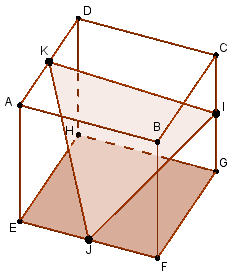
\includegraphics[width=0.4\textwidth]{01}
\end{figure}
\tabb1{\(\sqrt2\)}{\(\sqrt3\)}{\(2\)}{\(\sqrt5\)}
\newpage

%
\prob{07-기초2}
그림과 같이 모든 모서리의 길이가 \(6\)인 정사면체 \(D-ABC\)를 점 \(A\)를 원점에 \(B\)를 \(x\)축 위에, \(C\)를 \(xy\)평면 상의 1사분면 위에 있도록 좌표공간에 놓았다.
점 \(D\)의 좌표가 \((a,b,c)\)일 때, \(a^2+b^2+c^2\)의 값은?
\begin{figure}[h!]
\centering
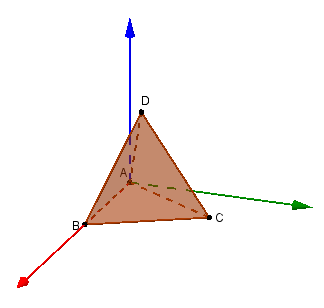
\includegraphics[width=0.4\textwidth]{02}
\end{figure}
\tabb{\(12\)}{\(18\)}{\(24\)}{\(30\)}{\(36\)}

%
\prob{07-기초3}
좌표 공간에서 두 점 \(A(3,4,-2)\), \(B(a,b,c)\)에 대하여 선분 \(AB\)를 \(2:3\)으로 내분하는 점이 \(x\)축 위에 있고, \(3:2\)로 외분하는 점이 \(yz\)평면 위에 있을 때, \(a+b+c\)의 값은?
\tabb{\(-5\)}{\(-4\)}{\(-3\)}{\(-2\)}{\(-1\)}

%
\prob{07-기본1}
좌표공간에서 선분 \(AB\)의 \(xy\)평면 위로의 정사영의 길이가 \(\sqrt{10}\), \(yz\)평면 위로의 정사영의 길이가 \(\sqrt5\), \(zx\)평면 위로의 정사영의 길이가 \(\sqrt{17}\)일 때, 선분 \(AB\)의 길이는?
\tabb{\(4\)}{\(\sqrt{17}\)}{\(3\sqrt2\)}{\(\sqrt{19}\)}{\(2\sqrt5\)}

%
\prob{07-기본2}
좌표공간의 두 점 \(A(1,6,1)\), \(B(-2,2,0)\)에 대하여 \(xy\)평면에서 점 \(B\)를 중심으로 하고 \(x\)축과 \(y\)축에 모두 접하는 원 위의 점을 \(P\)라고 하자.
선분 \(AP\)의 길이의 최댓값은?
\tabb{\(\sqrt{47}\)}{\(4\sqrt3\)}{\(7\)}{\(5\sqrt2\)}{\(\sqrt{51}\)}

%
\prob{07-실력1}
그림과 같이 좌표공간에 밑면인 원의 반지름의 길이가 \(1\)이고 높이가 \(2\)인 3개의 원기둥 \(S_1\), \(S_2\), \(S_3\)가 한 쪽 밑면이 모두 \(zx\)평면 위에 있도록 놓여있고, 밑면의 중심의 \(x\)좌표와 \(z\)좌표는 모두 양수이다.
\(zx\)평면에 속해 있는 \(S_1\)의 한쪽 밑면은 \(z\)축과 \(x\)축에 모두 접한다.
\(zx\)평면에 속해있는 \(S_2\)의 한쪽 밑면은 \(x\)축과 \(S_1\)의 밑면에 접하며, \(S_3\)의 밑면은 \(S_1\)의 밑면과 \(S_2\)의 밑면에 모두 접한다.
\(zx\)평면에 속해 있지 않은 \(S_3\)의 한쪽 밑면의 중심의 좌표를 \(P\)라고 하고, \(P=(a,b,c)\)일 때, \((a-b+c)^2\)의 값을 구하시오.
\begin{figure}[h!]
\centering
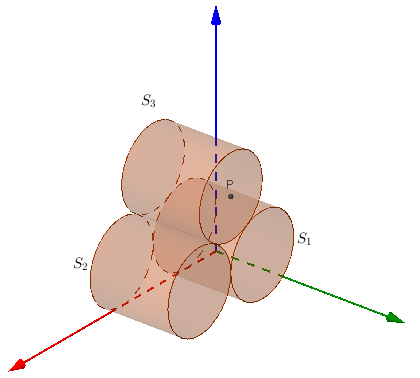
\includegraphics[width=0.6\textwidth]{03}
\end{figure}
\tabb{\(2+\sqrt{3}\)}{\(2+2\sqrt{3}\)}{\(4+\sqrt{3}\)}{\(4+2\sqrt{3}\)}{\(4+4\sqrt{3}\)}

%
\prob{07-실력2}
좌표공간의 세 점 \(A(1,2,3)\), \(B(5,-2,1)\), \(C(2,2,6)\)에 대하여, 두 점 \(A\), \(B\)에서 같은 거리에 있는 \(xy\)평면 위의 점 중에서 점 \(C\)까지의 거리가 최소인 점을 \(P\)라고 할 때, 선분 \(OP\)의 길이는?
(단, \(O\)는 원점이다.)
\tabb{\(2\sqrt2\)}{\(3\)}{\(\sqrt{10}\)}{\(\sqrt{11}\)}{\(2\sqrt{3}\)}

%
\prob{07-실력3}
[그림1]과 같이 한 변의 길이가 \(4\)인 정사각형 \(ABCD\)에서 선분 \(AB\)의 중점을 \(M\), 선분 \(BC\)의 중점을 \(N\)이라고 하자.
[그림2]는 정사각형 \(ABCD\)를 선분 \(MN\)을 접는 선으로 하여 두 평면 \(BMN\)과 \(AMNCD\)가 수직이 되도록 접어서 만든 도형이다.
이때 선분 \(BC\)의 길이를 구하시오.
\begin{figure}[h!]
\centering
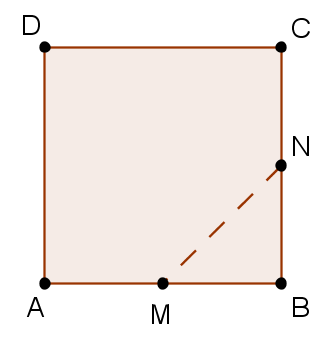
\includegraphics[width=0.3\textwidth]{04-1}
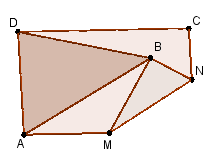
\includegraphics[width=0.3\textwidth]{04-2}
\par [그림1]\qquad\qquad\qquad\qquad[그림2]
\end{figure}
\tabb{\(\sqrt{10}\)}{\(\sqrt{11}\)}{\(2\sqrt{3}\)}{\(\sqrt{13}\)}{\(\sqrt{14}\)}
\newpage

%%%%
\begin{table}[h!]
\begin{tabular}{|c|c||c|c||c|c||c|c|}
\hline
\pn&\ding{175}	&\pn&\ding{174}	&\pn&\ding{176}	&\pn&\ding{176}\\\hline
\pn&\ding{172}	&\pn&\ding{175}	&\pn&\ding{175}	&\pn&\ding{174}\\\hline
\pn&\ding{174}	&&				&&				&&\\\hline
\end{tabular}
\end{table}

\end{document}